% this sections containes all the references for each section : 

% 1. group articles by field 


Efficiency in energy usage is a well-known topic. In the majority of fields, the purpose is to minimize the energy consumption of electrical devices/components. Modern times even see energy classification (A, B,... F) for Homes, cars and electronic products, to provide the consumer an indication of the energy consumption of his devices, which will reflect on his power bill. This creterions is extended even to the hardware components of computer.
figure\ref{fig:soa_comparaisoncpu} \footnote{\url{https://www.cpubenchmark.net/compare/Intel-i9-12900KS-vs-Intel-i9-12900KF/4813vs4611}}


\begin{figure}
    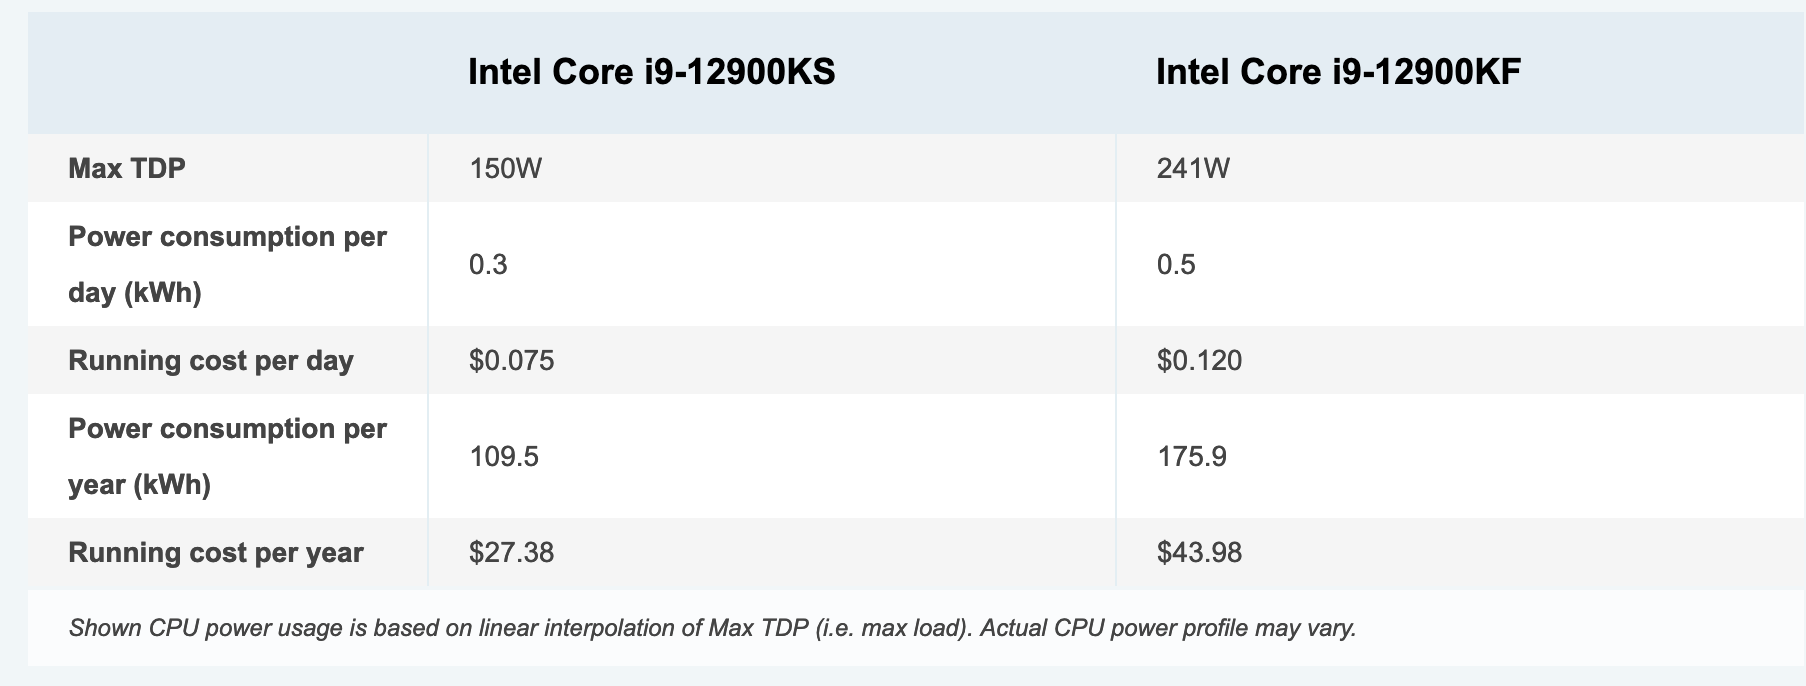
\includegraphics[width=\linewidth]{imgs/cpu_cost_comparaison}
    \caption{electrical cost comparasion between two cpus }
    \label{fig:soa_comparaisoncpu}
\end{figure}

In computer science, the objective is essentially same.
Numerous studies have been conducted on energy optimization.
Some of these studies concentrate on minimizing energy consumption at the hardware level, while others optimize energy consumption via software.
% displays the digital energy consumption distribution in 2017 \cite{andrae2015global}. ("p" for production and "u" for usage). 
% It demonstrates that both the production and consumption stages have substantial effects.
% In addition, the utilization expenses of data centers, networks, and terminals are also substantial (19 percent , 16 percent and 20 percent respectively).
% TODO : ask romain about the graphics for energy distribution 

As an example \citeauthor{avgerinou2017trends} evaluated the development of power use effectiveness (PUE) in data centers thkat belongs to various organizations participating in the European code of conduct for energy efficiency program \cite{avgerinou2017trends}.
The research found a gradual decline in the PUE of data centers, which measures the ratio of the overall energy supplied to the energy used by IT equipment.
A low PUE implies that the majority of energy is utilized to power the data center's IT equipment, while just a little amount is needed for cooling and lighting.

we will place a greater emphasis on the software level in order to decrease the amount of energy that is used.more particularly on the execution phase of the program cycle.
We will be proceeding through an empirical analysis of the energy consumption of the software while changing some components of the source code without impacting its behavior.
In order to do this, we will elaborate a benchmarking process and a set of tools that are intended to assist practitioners in better comprehending and optimizing the energy usage of their applications.
Thus, we will begin by examining the state of the art of empirical analysis and retrieving the best empirical experimentation methodologies in the research field.Then, we will narrow these practices down to computer science so that we can finally adapt them to energy consumption.

Section~\ref{sec:soa_benchmarking} will discuss the pitfalls and best practices associated with empirical research before applying them to our field of interest.
After that Section~\ref{sec:energymeasurement} describes software energy measurements.
It provides examples of hardware and software measuring instruments and describes their differences, benefits, and drawbacks. It also examines the sources of energy measurement variations, which represent a significant obstacle to achieving precise readings and a higher accuracy.
Then, in section \ref{section:soa_optimization}, we will go through some of the previous work on improving the energy consumption of softwares.

\newpage
\section{benchmarking}\label{sec:soa_benchmarking}
This section will go through the flaws and best practices of empirical research before applying them to our topic of study.

% We first start by defining the word \textbf{benchmark},  
% definition :benchmark: [noun] something that serves as a standard by which others may be measured or judged.
% that serves as a basis for evaluation or comparison (as of computer system performance)
In their work~\cite{van_der_kouwe_benchmarking_2018}, \citeauthor{van_der_kouwe_benchmarking_2018} Investigated 50 papers published in top venues
to findout that tier-1 papers commit an average of five benchmarking crimes.
To analyze the magnitude of the phenomenon, they have identified a set of 22 "benchmarking crimes" that threaten the validity of the system.
% TO [ROMAIN] should i include  this list ? 
% thoes benchmark crimes that one can commit intentionally or by accident and that could jeopardize the integrity of their paper.t are listed below.
% \begin{itemize}
%     \item  Not evaluating potential performance degradation
%     \item  Benchmark subsetting without proper justification
%     \item  Selective data set hiding deficiencies
%     \item  Microbenchmarks representing overall performance
%     \item  Throughput degraded by x\% => overhead is \%
%     \item  Creative overhead accounting
%     \item  No indication of significance of data
%     \item  Incorrect averaging across benchmark scores
%     \item  Benchmarking of simplified simulated system
%     \item  Inappropriate and misleading benchmarks
%     \item  Same dataset for calibration and validation
%     \item  No proper baseline
%     \item  Only evaluate against yourself
%     \item  Unfair benchmarking of competitors
%     \item  Not all contributions evaluated
%     \item  Only measure runtime overhead
%     \item  False positives/negatives not tested
%     \item  Elements of solution not tested incrementally
%     \item  Missing platform specification
%     \item  Missing software versions
%     \item  Subbenchmarks not listed
%     \item  Relative numbers only
% \end{itemize}



%% BENCHMARKING FRAMEWORK -- ADD IT later \cite{sonnenwald2003evaluating}
%further references 
In the book "Measuring computer performance: a practitioner's guide"\cite{lilja2005measuring},\citeauthor{lilja2005measuring} examines performance indicators and gives in-depth treatment of benchmark program tactics. He provides clear explanations of the basic statistical methods required for interpreting measured performance data. He also outlines the overall 'design of experiments' method and demonstrates how to collect the most information with the least amount of work. This practical book will appeal to anybody seeking a comprehensive, yet intuitive, grasp of computer system performance analysis.
\citeauthor{mytkowicz2009producing} made an evaluation  of 133 studies from ASPLOS, PACT, PLDI, and CGO, to find out that none of the experimental findings papers appropriately considered measurement bias. Which can lead derive incorrect results from an experiment if a seemingly insignificant feature of the experimental design is altered. They treated this problem by proposing two strategies for detecting measurement bias by using causal analysis and preventing it with setup randomization \cite{mytkowicz2009producing}.
\citeauthor{bukh1992art} wrote a book about computer performance analysis, where he discussed some familiar topics that are relevant to statistical analysis, such as null hypotheses, chi squared tests, regression, discrete event simulation, Bayes' theorem, how and when to use them for experimental design, measurement, simulation, and modeling for computer systems .





% further references 

%%%%%%%%%% 
In their paper~\cite{buytaert_statistically_nodate},\citeauthor{buytaert_statistically_nodate} they separated the start-up measurement from the steady state when comparing different Java optimizations.
\\
%\\\ https://www.cpubenchmark.net/compare/Intel-i7-12700KF-vs-Intel-i7-12700F/4608vs4692 | hardware benchmarking 
\section{energy measurement}\label{sec:energymeasurement}



to be able to reduce the energy cost of running programs we should first be able to estame this energy consumption.
many studies have been conducted to estimate a such energy consumption. that varries from static analysis of the source code to enfere it's energy consumption like \citeauthor{pereira_helping_2017} where they provided a tool to highlight the most energy consuming parts of the code \cite{pereira_helping_2017}.the main advantage of this apporach is to be able to estimate the energy consumption of a program without running it. however. unlike the conplexity of programs, the energy consumption is highly related the execusion environment. Therefor, Static analysis might not represent the real behaviour of the same program when it is run in the production environment.
To treat the problem of representativeness, many researchers tend to measure the energy consumption of the programs while they are running them. Hence we will get more accurate results.
there is a variety of tools to measure such energy, and they cover a large spectrium of usage depends on how \textbf{accurate} and \textbf{pricise} those results are needed to be in tone hand, and the price that practinoners are ready to pay for a such accuray/pricision.
Below we will present some tools that are well known in the literature and discuss their main advantages / drawbacks for our case.
\subsection{hardware tools}

% TODO Add : diagram of the possible point where we can measure the energy 

% depends on the scientific usage there are two apporaches :
% 1. extern one or independent : when the most of researchs are using
% the benifits of this is the simplicity of instalation however we pay the price either with a lack of temporal resolution ( low frequency ) or the spatial granularity
% ( most of them measure the energy consumption of the whole machine )
% 2. dedicated one , they are based on the instrumentation of some parts of the computer , however they have a high cost and they are defficult to scale since they require an instrumentation of the execusion environment.
according to \citeauthor{hackenberg2014hdeem} there are four main creterions to evaluate an energy measurement tool \cite{hackenberg2014hdeem}
\begin{itemize}
    \item \em{spatial granularity}: the more specific the target of monitoring we are able to measure, the more efficient we can do optimization since we will know what causes the pitfalls of the energy consumption.
    \item \em{temporal granularity}: same as spatial granularity, temporal granularity helps us to identif the sequence of code that need to be optimized.
    \item \em{scalability}: this is mainly related to the cost of the tools and the ease of their integration for our system.
    \item  \em{accuracy}:to elimanate extra hazards and get more representative measurement.
\end{itemize}

We believe that accuracy can be extracted from those creterions since it is a result of the combaination of the two first ones. therefore, we will focus more on the first 3 creterions from later on.
In the follwong section we will discuss some of the well known tools that are used in literature.


Nowdays, most of the high performance computing systems (HPC) implements a tool to report the energy consumption of the nodes for the sake of monitoring and administration. Those tools are mainly integrated withing the power suply units (PSU) or the power distributuin units (PDU). then , they provide an interface and a log to follow the history of the energy consumption. Despite their scalability and ease of integration. such tools lack both in spatial and temporal granularity since they monitor the whole energy of the nodes, and most of the times they have a very low sampling frequency. most of those tools are provided directly by the manufacturers. such as \em{IBM EnergyScale technology} \cite{mccreary2007energyscale} \cite{caldeira2014ibm} \cite{caldeiraibm} or \em{Dell poweredge} \cite{lovicott2009thermal}, MEGware Cluststafe \cite{breitbart2015case}
As we said earlier the true purpose of those tools is more monitoring than analysing the energy consumption.
%% add something to link with wattsup pro 
WattsUp Pro, is a device that can be installed  between the  powerer source of the machine and the system under test. it allows a sampling frequency up to 1Hz and has a internal memory to store a wide variety of data, such as the maximum voltage, current.. etc that later can be exported via USB port for personal usage or lined to some graph programs like Logger Pro or LabQuest.The main advantage of this tool is the ability to monitor the energy consumption from a different device which will reduce the risk of interference with the energy consumption of the test % a revoir 
\cite{hirst2013watts}

despite his high temporal granularity  , wattsup pro lacks in term of spatial granularity since it monitors the energy consumption of the whole system.
To have a finer granularity we need to isolate the energy consumption of each component.
.
For this we will need more intrusive tools such.

%% THIS IS FOR GPU %%% 
% GPU TESLA \cite{burtscher2014measuring}

% NVML\cite{fahad2019comparative}
%%%% 

PowerMon and its upgradded version powerMon2 \cite{bedard2010powermon} are based on an microcontroler chip that can monitor up to 6 channel ( 8 for powermon2) simultanetly. therefore we are able to monitor the powerconsumption of 4 devices at the same time. the frequency sample of this tool is up to 50Hz with an accuracy of 1.2\%. Powermore2 comes with smaller size that can fit within 3.5 inches rack drive.

PowerInsight \cite{laros2013powerinsight} is another finegrained measurement tool that is based on an ARM bagelbone processor \cite{coley2012beaglebone} which is able to measure up to 30 channel simultanetly with a frequency of 1KHz per channel.

on the other hand GreenMiner \cite{hindle2014greenminer}, %%i dont think that  mobile measurement will be relevent for my case 

powerpack \cite{ge2009powerpack} in the other hand is an api that synchronizes the data gathered from other monitoring tools such as Watt’s Up Pro, NI and RadioShack pro and the lines of code %% maybe remove this one from the list because it is not well known.

other monitor tools have been relized by the manufactures such as IBM Power executive \cite{koomey2011growth} which allows their customer to monitor the power consumption and thermal behaviour of the of BladeCenter systems in the datacenter.



%% TODO : add diagram where the distribution of the energy consumption is more related to the CPU rather than other tools - u can cite the tools dedicated to the GPU since it is is included in the software aggregators ? power api, pythoules ...etc 

as we see in % two diagrams one for research the other one for power usage 
The CPU is the part responsible of the most energy consumption of softwares. hence the finner we go to measure this energy consumption the better it is for our work.
Fortunately, Intel and later AMD proposed a tool that estimate the power consumption of different part of the CPI based on counter performances. RAPL (RUnning Average Power Limit) \cite{hackenberg2013power} \cite{hackenberg2015energy} is a set of registers that was introduced by intel in their CPU since Sandy bridge generation, and later it was fllowed by AMD since Family 17h Zen.
It is capable of monitoring different components of CPU , such as DRAM, Cores , and the integrated GPU for desktop processors.

%% TODO :ADD figure of RAPL + references 

The advanage of a such apporach is that the absence of any intrusive measurement tools. further more they have a high temporal granurality with a sampling frequency up to 1KHz \cite{ilsche_power_2015}.

with similar approach we can find NVIDIA reporting tools such as GPU TESLA \cite{burtscher2014measuring} and the NVML library \cite{fahad2019comparative}

\subsection{software tools}

Software-based measurement tools are based on other hardware tools to monitor energy use. Granularity is the core value of these technologies, unlike hardware tools, which only provide the total energy usage of the system/component (computer, server, motherboard, etc.) for most cases. Because they are frequently constructed on empirical estimations and data learning methods, they drop in accuracy.

Many software measuring tools understand the behavior of a power model and provide estimates of energy usage. This model is then used to allocate the observed energy consumption among different execution entities, such as processes, control groups, threads, or even code lines.

The first examples of software measurement tools are PowerAPI~\cite{colmant2018next}, SmartWatts formula~\cite{fieni2020smartwatts} and selfWatts~\cite{fieni2021selfwatts}.
These tools collect global energy consumption measurements from RAPL and use other system events such as cache misses/hits and CPU frequency evolution (DVFS) via a sensor to construct a power model of the control groups (system control groups, docker containers, kubernetes pods, etc.) using a Ridge regression.
The model continuously learns and improves its precision of real-time energy usage data with a maximum frequency of 100 Hz.
The instrument has a decentralized, lightweight design.
Only the lightest sensors required for data collection and transmission are put into the monitored devices.
The SmartWatts formula is then executed on the primary server in order to construct the model that permits assigning the energy usage for each operating control group.
PowerAPI is only compatible with Linux on a bare-metal physical computer.
\\
WattWatcher~\cite{lebeane2015watt} is a multi-core power measuring framework that provides process-level energy measurements.
This program uses power models to predict process energy usage. It uses CPU events which are passed from the measured node to a model generator node in order to construct the power model. It works by combining a description of the CPU with a list of the hardware events through multiple calibration phases in order to build a robust model.


Joulemeter~\cite{kothari2009joulemeter,jagroep2017energy} is a Microsoft software that estimates the energy usage of Windows running applications down to the process level by using power models (for CPU, memory, and drives).
It employs low-overhead power models to infer power consumption from resource utilization during runtime, and it provides power limiting features for virtual machines.
Previous Joulemeter tests~\cite{jagroep2015profiling} demonstrated that the instrument provides a less accurate estimation of energy use that differs greatly from the real one.
To adjust its models to the hardware on which it operates, Joulemeter must first go through a calibration step.
It is able to only monitor one process at a time with a frequency of 1 HZ.



JRAPL is another example of an energy measurement tool estimating tool that has been utilized in a variety of publications\cite{guimaraes2016some,liu2015data}.
This software enables for the energy usage of Java programs, functions, or even a block of code lines to be profiled and measured.
The measurements are heavily reliant on the data supplied by RAPL.
As a result, the global energy consumption collected by RAPL between two timestamps (the start and finish of the code to measure) is used to calculate the energy consumption of the Java code.
Tests using JRAPL should be done on a well-configured machine to minimize the impact of the operating system and user operations on the overall energy consumption of JRAPL.

Another process-level energy usage measuring tool is Jolinar \cite{islam2016measuring,noureddine2016jolinar}.
The tool does not need a calibration phase and relies on pre-established power models based on hardware metrics (TDP, disk I/O rate, and so on).
These settings must be identified and supplied by the user for his machine.
Jolinar is only capable of measuring the energy consumption of one application at a time.
At the end of the execution, the tool provides the CPU, DRAM, and disk energy usage of the main process.
joulinar

Jalen\cite{noureddine2015monitoring} is another tool that profiles and monitors the energy usage of a Java program. Unlike JRAPL, Jalen is able to reduce the scope up to the function level.
It gathers data using code instrumentation and statistical sampling at a predetermined pace.
Because of the overhead that code instrumentation may incur, the authors recommend utilizing the second option.
Every 10 ms, Jalen records the JVM's stack trace together with the CPU time of threads and computes statistics about method calls.
These statistics are then utilized to calculate each method's energy usage.

selfwatts \cite{fieni2021selfwatts}
powerjoular \cite{noureddine2022powerjoular}

\subsection{hybrid tools}
% split hardware tools into extern and embeded tools 

Simgrid simulation of power consumption of parallel aplication using simgrid \cite{heinrich2017predicting}

impact of manifacturing process on the energy variation \cite{coles2014comparing}

different energy consumption between identical processers [ idle and hight load ]\cite{von2016variations}

the temperature is the main raison a high energy variation \cite{wang2018potential}

external factors are impact on the energy variation \cite{mukherjee2009spatio}

the place of the server in the room doesn't affect the energy variation \cite{diouri2013your}

comparaison of three measuring tools and they did exhebit 10\% variation each time \cite{inadomi2015analyzing}

%%****** mitigating the energy variation ******
low-cost scalable variation-aware algorithm \cite{inadomi2015analyzing}

reducing the energy variation by disabling turbo boost \cite{acun2016variation}

reducing the energy consumption in parallel systems \cite{chasapis2016runtime}

\cite{marathe2017empirical}



\section{programming languages and performances}\label{section:soa_optimization}
\subsection{energy}\


energy comparaison of programming languages in the game benchmark by debian \cite{pereira2017energy}

toward green ranking \cite{couto2017towards}

java vs kotlin in web performances \cite{bujnowski2020java}

rosetta code \cite{nanz2015comparative} \cite{mirowski2020rosetta}

network energy comparaison \cite{balasubramanian2009energy}

Aequitas \cite{ribic2016aequitas}

vm placement \cite{mishra2018energy}

\citeauthor{mishra2018energy}

static cost of Vms \cite{kurpicz2016much}



carbon footprint of training neural network \cite{strubell2019energy}

SPELL, the energy leaks detector tool \cite{pereira2017helping}

impact of energy profiling on software \cite{jagroep2017energy}

impact of maintability on software energy evolution \cite{calero2021does}

defintion \cite{wang1993grpc}

comparaison \cite{chamas2017comparing}

emprical study \cite{de2021empirical}

impact of website implemenation on energy consumption \cite{philippot_characterization_2014} \cite{manotas2013investigating}

PHP \cite{benmoussa_new_2019} \cite{das_comparison_2016}

simulation of web cache \cite{cardenas_performance_2005}

java spring analysis \cite{gajewski_analysis_2019}

performance \cite{mishra2021web}


cross compiler benchmarking \cite{yet2016cross}

\subsection{python}

webframeworks on python \cite{pankiv_concurrent_nodate}

hope library \cite{akeret_hope_2015}

bytecode effect \cite{ben_asher_effect_2009}

numba \cite{crist_dask_2016}

intel python \cite{li_boosting_2016}

python 2 vs 3 \cite{modzelewski_pyston_2020}

python runtime performances \cite{redondo_comprehensive_2015} \cite{murri_performance_2013}

static vs dynamic languages \cite{pang_what_nodate}

concurent benchmark framework \cite{pankiv2019concurrent}


\subsection{jvm}

java vs python \cite{destefanis_statistical_2016}

hotspot vs J9 \cite{oi2011power} - same but for big querries \cite{chiba2018towards}

constant overheat of the jvm \cite{lafond2006energy}

infer the energy cost based on the byte code instructions \cite{ma2017biogeography}

java collection energy footprint  \cite{pinto2016comprehensive} \cite{fernandes2017assisting}

java classes energy footprint \cite{hasan2016energy}

framework to reduce java collections \cite{manotas2014seeds}

energy consumption of java dev tools \cite{baskar2013experimental}

Microbenchmarks on jvm \cite{longo2019reducing} \cite{baskar2013experimental}

android automatic refactoring to reduce energy consumption \cite{banerjee2016automated} \cite{rodriguez2017reducing}

java vs native c in android \cite{corral2014method}





\subsection{benchmarking}
%%%%%%%%%%% further references 
NAS \cite{bailey_nas_nodate}
statistics \cite{he_statistics-based_2019}
benchmark crimes \cite{van_der_kouwe_benchmarking_2018}
microservices \cite{grambow_benchmarking_2020}
impact of webservers on web applications energy \cite{manotas_investigating_2013}
%%%%%%%%%%%%%%%%%  virtualisation 

%%%%%%%%%%%%% energy metigation 

\section{Energy Variation}
\subsection{Studying Hardware Factors}
This variation has often been related to the manufacturing process~\cite{coles_comparing_2014}, but has also been a subject of many studies, considering several aspects that could impact and vary the energy consumption across executions and on different chips.
On the one hand, the correlation between the processor temperature and the energy consumption was one of the most explored paths.
Kistowski~\emph{et~al.} showed in~\cite{joakim_v_kisroski_variations_2016} that identical processors can exhibit significant energy consumption variation with no close correlation with the processor temperature and performance.
On the other hand, the authors of~\cite{wang_potential_2018} claimed that the processor thermal effect is one of the most contributing factors to the energy variation, and the CPU temperature and the energy consumption variation are tightly coupled.

\note{add the corelation value}

This exposes the processor temperature as a delicate factor to consider while comparing energy consumption variations across a set of homogeneous processors.%, but also, if a same workload can cause the CPUs to reach different temperatures.

The ambient temperature was also discussed in many papers as a candidate factor for the energy variation of a processor.
In~\cite{ranka_energy_2009}, the authors claimed that energy consumption may vary due to fluctuations caused by the external environment.
These fluctuations may alter the processor temperature and its energy consumption.
However, the temperature inside a data center does not show major variations from one node to another.
In~\cite{el_mehdi_diouri_your_2013}, El~Mehdi~Dirouri~\emph{et~al.} showed that switching the spot of two servers does not affect their energy consumption.
Moreover, changing hardware components, such as the hard drive, the memory or even the power supply, does not affect the energy variation of a node, making it mainly related to the processor.
This result was recently assessed by~\cite{wang_potential_2018}, where the rack placement and power supply introduced a maximum of $2.8\,\%$ variation in the observed energy consumption.

Beyond hardware components, the accuracy of power meters has also been questioned.
Inadomi~\emph{et~al.}~\cite{inadomi_analyzing_2015} used three different power measurement tools: RAPL, Power Insight\footnote{\url{https://www.itssolution.com/products/trellis-power-insight-application}} and BGQ EMON.
All of the three tools recorded the same $10\,\%$ of energy variation, that was supposedly related to the manufacturing process.
%% this is to prove that the problem is REAL !!! 

\subsection{Mitigating Energy Variations.}
Acknowledging the energy variation problem on processors, some papers proposed contributions to reduce and mitigate this variation.
In~\cite{inadomi_analyzing_2015}, the authors introduced a variation-aware algorithm that improves application performance under a power constraint by determining module-level (individual processor and associated DRAM) power allocation, with up to $5.4\times$ speedup.
The authors of~\cite{hammouda_noise-tolerant_2015} proposed parallel algorithms that tolerate the variability and the non-uniformity by decoupling per process communication over the available CPU.
Acun~\emph{et~al.}~\cite{acun_variation_2016} found out a way to reduce the energy variation on Ivy~Bridge and Sandy~Bridge processors, by disabling the Turbo~Boost feature to stabilize the execution time over a set of processors.
They also proposed some guidelines to reduce this variation by replacing the old---slower---chips, by load balancing the workload on the CPU cores and leaving one core idle.
They claimed that the variation between the processor cores is insignificant.
In~\cite{chasapis_runtime-guided_2016}, the researchers showed how a parallel system can be used to deal with the energy variation by compensating the uneven effects of power capping.

In~\cite{marathe_empirical_2017_m}, the authors highlight the increase of energy variation across the latest Intel micro-architectures by a factor of $4$ from Sandy~Bridge to Broadwell, a $15\,\%$ of run-to-run variation within the same processor and the increase of the inter-cores variation from $2.5\,\%$ to $5\,\%$ due to hardware-enforced constraints, concluding with some recommendations for Broadwell usage, such as running one hyper-thread per core.
%  NOTE :/this might be interesting for greeFaaS





\section{Conclusion}
As we have seen in the state of the art, many methodes have been proposed to reduce the energy footprint of the the ICT,which they can be applied in deffirent parts of the lifecycle of the program, from consumption to the execution. Furthermore, the execution phase took attention of many researchers because it's the part where the most energy is consumed. This thesis will focus on that aspect as well. However, unlike the most work that have been done on the hardware aspect, we will target the software impact on this energy, starting from the choice of the programming language up to how to tune some features of a frameworks in order to make the software consumes less energy.To do so we use the emprical apporach due to it's concinstency for the moment.Unlike the perfromance which essentialy related to the complexity of the algorithm, the energy consumption is more impacted by the hardware.
Therefore, to optimize the enrgy consumption we choose a spiral methode. based on 3 phases:
\begin{enumerate}
    \item execute the code
    \item measure the program
    \item infere the guidelines
\end{enumerate}


\begin{figure}[!hbt]
    \center{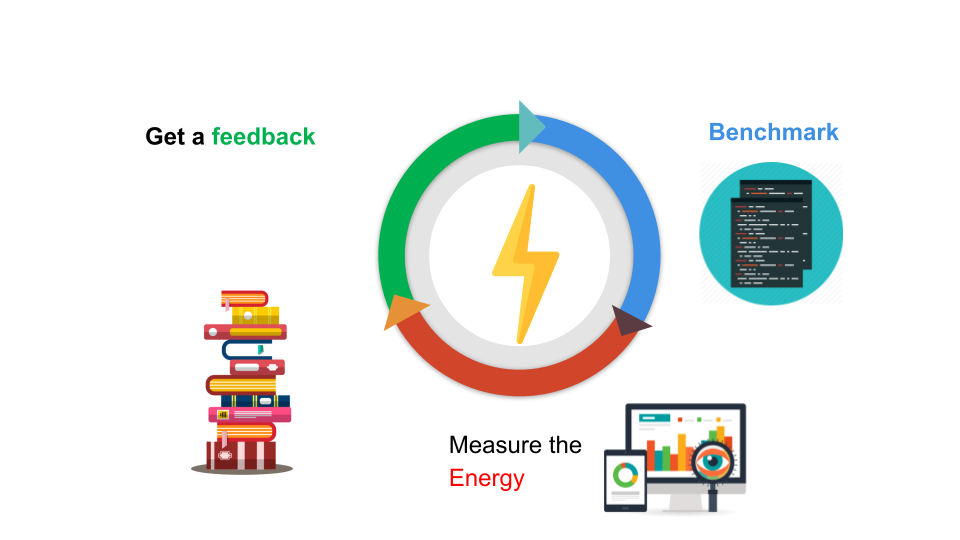
\includegraphics[scale=0.3]{imgs/greenbenchmarkcycle}}
    \caption{the spiral methode of energy optimization }\label{fig:spirals}
\end{figure}
the aim of this work is to present a set of guidelines to create a benchmarking system to to measure the energy consumption of different programs.
After that, we will use this system to compare the energy consumption of different programming languages. We will extend the work of \citeauthor{pereira2017energy} to a closer distance to production environment by comparing a set of usecases. starting by GRPC framework, and a set of Web Framewroks. Finally we will discuss the impact of the execution environment on the energy consumption of two of the most famous programming languages JAVA and Python. and present how can tunning the Virtual Machine can reduce the energy consumption.

